% \documentclass{article}
\documentclass[twocolumn]{article}
\usepackage{graphicx} % Required for inserting images
\usepackage{amsmath}
\usepackage{amssymb}
\usepackage{mathtools}
\usepackage[backend=biber,style=numeric]{biblatex}
\addbibresource{citations.bib}

\title{Hexagons are the Bestagons: A Novel Neural Network Topology}
% \author{Daniel Lopez, Cezareo Rodriguez}
\author{
Daniel Lopez \quad Cezareo Rodriguez\\
SimpleRose Inc.,\\
St. Louis, MO\\
\texttt{\{daniel, cezareo\}@simplerose.com}
}


\date{May 2026}

\begin{document}

\maketitle

\begin{abstract}
    We propose and establish baselines for a novel, albeit impractical neural network topology that departs from traditional Cartesian grid layouts of neurons and connections and employs a hexagonal lattice enabling neighboring networks with overlapping weights, Hexagonal Neural Networks.
    Inspired by extreme behavior compartmentalization behavior disorders observed in the general populace, this network structure focuses on the influence of directional training on overlapping weights.
    Early baselines reveals new learning behaviors through loss and accuracy iterations and consistent improvement from single direction propagation which has widespread usage in modern day commercial deep learning structures.

    %%% SUGGESTION: The abstract currently mixes architectural claims, cognitive motivation, and empirical observations together. For a stronger conference paper, consider narrowing the abstract to:
    %%% SUGGESTION: (1) what HexNNs are,
    %%% SUGGESTION: (2) what experimental question is tested,
    %%% SUGGESTION: (3) the strongest observed result.
    %%% SUGGESTION: Existing text: "Inspired by extreme behavior compartmentalization behavior disorders..."
    %%% SUGGESTION: This is likely too speculative for the abstract. Move human/cognitive inspiration to a short motivation paragraph or omit from the conference version.
\end{abstract}

\section{Introduction}

Multilayer perceptrons are traditionally structured as a unidirectional chain of fully-connected layers, where each layer only connects to the next in sequence.
While this base model has had several iterations that are found in modern day powerful AI systems, most commercial systems stick to this linear direction of deep learning, given how well this can scale.
Significant progress has been made on this front as geometric deep learning has explored architectures that are robust to different transformations of data.
For example, they are invariant to affine transformations such as translation, rotation, scaling.

However, the expressive potential of neural computation may not be limited to such linear structures.

Arbitrary Neural Networks, for example, have sparse research surrounding it since they are impractical for scaling in terms of memory, unstructured layers, and time for experimentation.
More heavily researched architectures, however, include group equivariant CNNs, spherical CNNs, and message passing neural networks in efforts to incorporate symmetry into neural processing.
Specifically, the filters that are used in convolution layers are rotated for angular invariance of features in the context of image recognition.
While this symmetry tends to help the network stay robust in equivariance of the system, it still is a single network in a linearly trained direction.

Borrowing from this tradition of symmetry, but allowing multidirectional tiling and directionality, consider a Hexagonally constructed neural network.
We can preserved bipartite connections between layers to retain the fully connected nature of MLPs, but we can gain rotation redundancy of hexagonal tilings, and expose two more networks with shared weights.
Here, we introduce Hexagonal Neural Networks (HexNNs) that may generalize MLP into a rotationally symmetric, multi-directional structure.

HexNNs replace the standard 1D layer stack with an initial 2D topological arrangement made to resemble regular hexagons.
Given a size parameter, $n$, the network has equal $n$ length input and output layers, with hidden layers symmetrically increasing and decreasing to $2n-1$.
Crucially, each node in layer $i$ is connected to all nodes in layer $i+1$, but unlike MLPs, this bipartite adjacency is true for all three cardinal directions of a hexagon.
This allows for rotation-based reinterpretation of the network's directionality.

This design enables six distinct orientations of the same network, each corresponding to a $60^\circ$ rotation of the hexagonal structure.  
We define each orientation as a subset of the network, $H_i$, and note that forward propagation of any $H_i$ is equivalent to backwards propagation of its  corresponding opposite network, $H_{(i+3) \bmod 6}$.

\subsection{Open Questions}
This architectural symmetry leads to several research questions that can uniquely be defined by this structure, but primarily: \textit{if we train a hexagonal neural network, what impact does that have on the performance of the networks in other directions?}

%
% TODO: write the below as more questions
%

% Things we can mess with:
% - alternate training (learn h1, h2, h3, then delta W? or learn all h1, then delta w then all h2, then delta w, then all h3, and then delta w)

% - training in h1, messes with training in h2, and h3, how?

% - are some directions more 'learnable' than others due to asymmetries in initialization or dataset alignment?

% - what structural features emerge in the weight matrix when optimzated for ALL SIX directions simultaneously

\section{Background}

\subsection{MLPs and Layered Function Approximation}
% Points to hit:

% MLPs as compositions of affine transformations and nonlinearities.
% Standard feedforward directionality.
% Fully connected adjacent-layer transformations.
% This HexNN keeps this adjacent-layer bipartite assumption but changes the topology/directional interpretation.

MLPs can be described as a composition of affine transformations and (typically) non linear activation functions.
Iterations on derivative architectures modify this basic pattern with tricks like weight sharing, recurrence, attention blocks, or structured sparsity.
However, they still maintain the feedforward directionality of the network.

Moreover, standard dense MLPs are not able to encode more complex inductive biases such as rotational invariance or translational invariance by themselves.
These biases must be introduced through some creative license on network features like architecture, data representation, or training procedure.

HexNNs, as introduced in this paper, keeps this adjacent-layer bipartite structure from MLPs but changes its own topology to allow for multiple feedforward interpretations from the same graph, potentially allowing for more complex inductive biases.

\subsection{Symmetry and Equivariance in Neural Networks}
% Points to hit:

% CNNs encode translational structure.
% Group-equivariant CNNs encode transformations such as rotations/reflections.
% Spherical CNNs extend symmetry ideas to spherical domains.
% Your project differs because:
% the symmetry is imposed on the network topology, not only the input domain or filter group,
% the same node/weight structure can be reinterpreted directionally.

Convolutional Neural Networks (CNNs) are a prime example of how the architural constraints of the input domain can be used to encode more complex inductive biases.
They encode translational equivariance and locality of features in the input data by using convolutional filters that are "slid" across the input data.
Their derivative architecture use geometric iterations on their kernels and inputs to help them unlock higher level inductive biases:
Group-equivariants CNNS encode the symmetry of the input data itself to achieve rotation, reflection, or other group equivariances equivariance and Spherical CNNs extend the symmetry ideas to spherical domains for rotational equivariance.
Capsule Networks project their input data into higher dimensionality with their vector interpretaion and yield complex understandings of part-whole relationships in their latent space.

All of these architectures, however, still impose a feed forward directionality on the layer ordering.
In the case of HexNNs, the symmetry is imposed on the network topology itself, not only the input domain or filter group.
This allows for the same node/weight structure to be reinterpreted directionally with abstraction bleeding between the different directions.

% \begin{table*}
%     \centering
%     \begin{tabular}{c|c|c}
%         Architecture & Key Difference from MLP & Inductive Biases \\
%         \hline
%         \hline
%         CNN & Convolutional Filters & Translational equivariance; Locality \\
%         \hline
%         RNNs (LSTMs, GRUs, etc.) & Recurrent Connections & Equivariance to Temporal Ordering; Statefulness; Causal Structures \\
%         \hline
%         Transformers (BERT, GPT, etc.) & Attention Mechanism & Permutational invariance; Global Context; Scalable Attention; Self-Attention \\
%         \hline
%         GNNs (GraphSAGE, GAT, etc.) & Message Passing & Graph Structure \\
%         \hline
%     \end{tabular}
% \end{table*}

\subsection{Graph Neural Networks}
% Points to hit:

% GNNs operate over graph-structured data.
% Message passing uses adjacency to constrain information flow.
% HexNN can be described as a graph-structured feedforward network, but it is not necessarily a GNN unless you implement message-passing layers.
% This helps prevent reviewers from saying, “isn’t this just a GNN?”

% Important distinction:

% HexNN is graph-structured, but its current implementation is closer to a sparse/directed MLP with orientation-specific adjacency than to a conventional message-passing GNN.
Graph neural networks operate on data whose structure is represented by a graph. 
In message-passing GNNs, node representations are updated by aggregating information from neighboring nodes according to an adjacency relation. 

HexNNs also use an adjacency structure, but the present formulation differs from standard GNNs in two ways:
First, the graph defines the architecture itself rather than the input data. 
Second, computation proceeds through orientation-specific feedforward traversals rather than repeated permutation-invariant neighborhood aggregation. 
For this reason, the current HexNN implementation is better understood as a graph-structured or sparse MLP topology rather than a conventional message-passing GNN.


\subsection{Parameter Sharing, Ensembles, and Multi-Head Models}

% Points to hit:

% Ensembles improve robustness through diversity.
% Parameter sharing can reduce memory and couple learning.
% Multi-head/shared-backbone systems separate shared representation from task-specific output layers.
% HexNN can be interpreted as a parameter-sharing ensemble where directional subnetworks are geometrically coupled.

Parameter sharing is commonly used to reduce model size and impose structure. 
CNNs share kernels across spatial locations, recurrent networks reuse transition parameters across time, and multi-task models often share a representation backbone across related objectives. 
HexNNs use a different form of sharing: orientation-specific subnetworks are coupled through a common underlying graph. 
Training one orientation may therefore alter the behavior of other orientations, creating measurable transfer or interference.

HexNNs can also be compared with ensembles. 
Unlike an ensemble of independent models, a HexNN does not maintain separate parameters for each orientation. 
Its directional subnetworks are not independent; their behavior is coupled by construction.


\subsection{Continual Learning and Interference}

% Points to hit:

% Sequential learning can cause interference between tasks.
% Catastrophic forgetting is a known failure mode.
% Your experiment is not exactly continual learning unless you train orientations/tasks sequentially.
% The relevant concept is interference through shared parameters.

Moreover, human cognition and artificial intelligence are known to face common challenges, such as managing knowledge across diverse tasks without losing prior knowledge gain.
This is known as catastrophic forgetting, where a network trained on one task is unable to perform well on a different task.
This is a known challenge in artificial intelligence, and it is a known challenge in human cognition.


\subsection{Cognitive Motivation}
% Points to hit:

% Neural networks are historically brain-inspired abstractions.
% The HexNN structure was partly motivated by questions about compartmentalized behavior and shared internal representation.
% This paper does not model DID or human identity.
% The cognitive analogy is heuristic, not empirical.

Foundational architectural models that have been proposed are able to uncover different inductive biases that are not possible with the traditional MLP architecture using natural design as motivation.
CNNs, for example, discovered feature invariance after modeling the convolutional kernals after the visual cortex and its neurophysiological design.
RNNs and LSTMs resemble the neurophysiological self looping design of the hippocampus and its role in memory and spatial navigation and this was able to introduce the concept of recurrent connections and the idea of memory cells in artificial intelligence.
So consider the phenomenon found in people who have a dissociative identity disorder (DID), where memories and personalities are split between identities despite having the same brain.
To borrow speculative language from Douglas Hofstadter, we can imagine a network toplogy that is able to hold different representations of the same data in the same hardware and each "strange loop" working as its own coherent identity but potentially affecting the learned experiences with other identities.

%Philosophical accounts of self-reference and cognitive loops offer one informal motivation for considering architectures with multiple recurrent or directional interpretations, but the present work does not depend on those claims.

To be clear, this paper does not model DID or aim to benchmark DID like symptoms in a clear method like the research proposed by [blank].
DID was the human based inspiration given its similar characteristics to extremely compartmentalized behavior, something not usually found in highly emergent cognitive systems, such as humans.
This inspiration also comes from the primary author's own trauma with a mother with split identities, and a father with hemiplegia after a hemoraggic stroke impaired his ability to move his left side.
The cognitive analogy is strictly heuristic, not empirical.

\section{Implementation}

%%% SUGGESTION: For conference review, this section should read less like a narrative and more like a reproducible model specification.
%%% SUGGESTION: Recommended order:
%%% SUGGESTION: (1) topology and layer sizes,
%%% SUGGESTION: (2) orientation/layer indexing,
%%% SUGGESTION: (3) adjacency and weight masks,
%%% SUGGESTION: (4) forward pass,
%%% SUGGESTION: (5) training/update rule,
%%% SUGGESTION: (6) computational complexity,
%%% SUGGESTION: (7) implementation notes.
%%% SUGGESTION: Existing ensemble variants near the end may fit better in Benchmark Families or Future Work unless they are experimentally evaluated.

\subsection{Topological Definition}
A one directional view hexagonal neural network is a multilayer perceptron network whose layer sizes increase and then decrease symmetrically, forming a hexagon-like outline if it were to be drawn in 2D.
As expected, all neurons in any given layer are fully connected to all neurons in the subsequent layer.
However, due to the hexagonal nature of the framework, there are three distinct directions in which one could perform traditional forward and backward neural network propagation.
This renders the structure to contain a unique corresponding arrangement of connections and shared weights given the direction.

%%% SUGGESTION: Existing text: "three distinct directions"
%%% SUGGESTION: Clarify early that there are six orientations but three geometric axes if opposite directions share/reverse weights.
%%% SUGGESTION: Reviewers may otherwise see an inconsistency between "three distinct directions" and later $H_0, \ldots, H_5$.

These shared weights may influence the internal network's representation of data in their high-dimensional embedding from one propagation direction to another in strange ways.
The shared weights of, say, the first semantic layer of $H_1$ will always have at least one shared weight with $H_2$ (the relative leftmost neuron from $H_2$'s point of view) up until the halfway point of the network.
This overlap is small but non-neglible as these weights are now subject to the gradient descent paths of two distinct target local optimas.
Experimentally, we actually see equivalent or better another local optimum, outperforming the two original networks had they been started with the same random seed patterns for their respective weights across the benchmark set (detailed below).
Since each layer represents a layer of abstraction away from the input reality towards the target reality, it could be speculated that any one layer's abstraction has a cross abstractive coherence bias on another's direction and thus representation.

%%% SUGGESTION: Existing text: "strange ways"
%%% SUGGESTION: Replace with a measurable term such as "transfer", "interference", or "cross-orientation coupling".
%%% SUGGESTION: Existing text: "two distinct target local optimas"
%%% SUGGESTION: This is technically risky. Local optima claims are difficult to substantiate without loss landscape analysis.
%%% SUGGESTION: Consider describing this as "distinct optimization trajectories" unless you actually measure optima.
%%% SUGGESTION: Existing text: "Experimentally, we actually see..."
%%% SUGGESTION: Move empirical claims out of Implementation and into Results, then cite figure/table/run identifiers there.

\subsection{The Greek Stuff}

%%% SUGGESTION: Rename this subsection before submission.
%%% SUGGESTION: Options: "Formal Topology", "Layer-Size Definition", or "Notation and Geometry".

The layer sizes of a HexNet of a parameter size $n$ follow an explicit pattern:

\[L = [n, n+1, ... 2n-1, ..., n+1, n]\]

with a $2n-1$ total layers as well.
The total number of nodes in a network, however, is:

\[T = \sum_{k=0}^{2n-2} (n + \min(k, 2n-2-k))\]

%%% SUGGESTION: Consider adding the closed form $T = 3n^2 - 3n + 1$ if correct for your topology.
%%% SUGGESTION: This helps reviewers quickly reason about scaling.
%%% SUGGESTION: Also add parameter-count equations for:
%%% SUGGESTION: - one orientation path,
%%% SUGGESTION: - dense global matrix representation,
%%% SUGGESTION: - parameter-matched MLP baseline.

\subsubsection{Weight Indexing and Layer Sets}

To be explicit, if we visualize the network with the layers centered and stacked vertically (i.e. with the smallest layers at the top and bottom, widest in the middle), then we have the following directions:
\begin{itemize}
    \item \textbf{$H_0$:} Top-to-bottom layers (default hexagonal structure)
    \item \textbf{$H_1$:} Top-right to bottom-left diagonal
    \item \textbf{$H_2$:} Bottom-right to top-left diagonal
    \item \textbf{$H_3$:} Bottom-to-top layers (reverse of $H_0$)
    \item \textbf{$H_4$:} Bottom left to top-right diagonal
    \item \textbf{$H_5$:} Top left to bottom-right diagonal
\end{itemize}

%%% SUGGESTION: Verify this orientation labeling matches your code and figures exactly.
%%% SUGGESTION: Inconsistency between diagrams, code, and notation will be heavily punished by reviewers.
%%% TODO: add a table mapping orientation labels to code rotation IDs and geometric direction.

\subsubsection{Global W}

For mathematical simplicity, we employ a global weight matrix $W$, a adjacency matrix of size $T x T$ that can represent all possible connections regardless of rotation.
Given that $H_0$ is directionally opposite $H_4$, they would share exactly the same weights.
While empirical trials on MLPs show that bidirectional training on the same weights show catastrophic loss, (find reference), we could theoretically use different cells to represent that as a separate network and still maintain directional-abstraction bleeding between immediately neighboring dimensions.
If this were the case, then $W$ would not be symmetric.
An example of this is shown in Figure \ref{fig:hexnet_n3_multi_activation}.

%%% SUGGESTION: Existing text: "$H_0$ is directionally opposite $H_4$"
%%% SUGGESTION: Earlier notation says the opposite orientation of $H_i$ is $H_{(i+3) \bmod 6}$, which would make $H_3$ opposite $H_0$.
%%% SUGGESTION: This needs correction before submission.
%%% SUGGESTION: Existing text: "bidirectional training on the same weights show catastrophic loss"
%%% SUGGESTION: This needs either a citation, a specific experiment, or removal. It currently reads as an unsupported empirical claim.
%%% SUGGESTION: Existing text: "directional-abstraction bleeding"
%%% SUGGESTION: Consider replacing with "cross-orientation parameter coupling".

\begin{figure}
    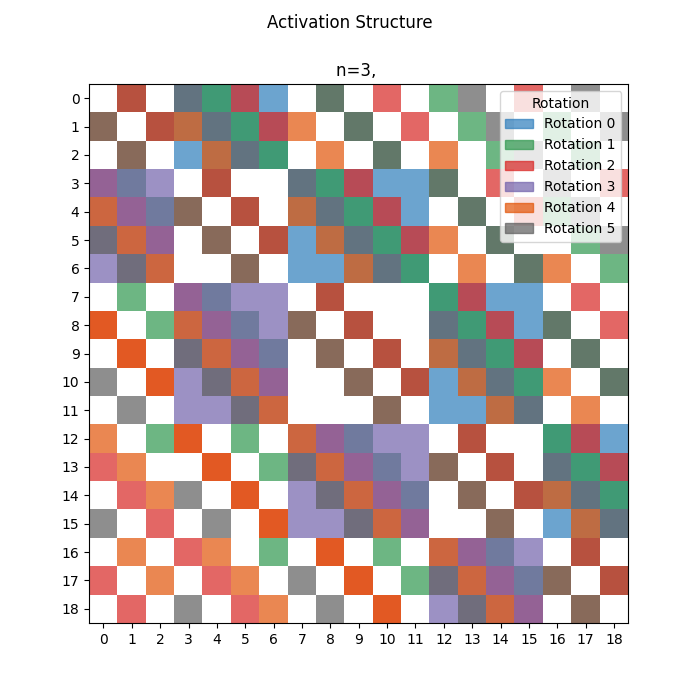
\includegraphics[width=1\linewidth]{hexnet_n3_multi_activation.png}
    \caption{Overlay of the orientation-specific adjacency patterns for a HexNN with n=3. Each color corresponds to one directed orientation.}
    \label{fig:hexnet_n3_multi_activation}
\end{figure}

\subsubsection{Directional W}
We can represent the static MLP view of any arbitrary rotation, $r \in {0, 1, 2, 3, 4, 5}$ as $W_i$ with a mask over $W$ enforcing a layered feedforward structure.

%%% SUGGESTION: Use $r \in \{0,1,2,3,4,5\}$ instead of $r \in {0, 1, 2, 3, 4, 5}$ for LaTeX correctness.
%%% SUGGESTION: Also clarify whether $W_i$ should be $W_r$, $W^{(r)}$, or $A^{(r)} \odot W$.

For the next few mathematical definitions, let the \textbf{Vertical Direction} orientation of the network, $H_1$, be the assumed direction.
Furthermore, let's assume the numbering of the network to start from the top left index, traverse left to right, and then top to bottom.
Let:
\begin{itemize}
    \item $A^{i} \in \{0, 1\}^{T \times T}$ be the binary adjacency matrix for arbitrary direction $H_i$
    \item For node index $i \in [0, T-1]$, let $\mathrm{layer}(i)$ map it to its layer number $l \in [0, N_{L}-1]$
    \item $S_{l}$ be the set of indices in layer $l$
\end{itemize}

%%% TODO: define $N_L$ before first use.
%%% TODO: define whether $A^i$ is directed or symmetric.
%%% TODO: define whether $W$ stores all possible directed edges or only canonical undirected edges.

\subsubsection{Directions as Rotations}
As previously noted, properties such as layer sizes and layer weights for $H_i$ will be the reverse for the geometric opposite network, $H_{(i+3) \bmod 6}$, and therefore, adjacency matrices, weight matrices, and other relevant matrices can all be considered symmetric (or at least will be in this paper).
But this now introduces rotation as a potentially active participant in the training steps.
Thus, for forward propagation, you can just iteratively compute:

\[x_{t+1} = R_k(f_d(W^T \times p_d(x_t)))\]

where $x_t$ is the latent vector at step $t$, $f_d$ is the hex net forward propagation through direction $d$, $R_k$ is the rotation operator at $k$, the selected rotation step, and $p_d is merely a padded mapping of x$

%%% SUGGESTION: This equation reads like a recurrent/orbit formulation, not the core feedforward implementation.
%%% SUGGESTION: If recurrence is not central to this conference paper, consider moving this to Future Work or clearly labeling it as optional rotational iteration.
%%% SUGGESTION: Existing text: "$p_d is merely a padded mapping of x$"
%%% SUGGESTION: Missing math delimiter around $p_d$ and $x$; also "merely" can be removed for technical tone.
%%% TODO: define the actual feedforward equation for a single orientation separately from iterative rotation experiments.

\subsubsection{Adjacency Matrices}

Then, the $H_1$, the only non-zero entries in $A$ are defined as:

\[A_{ij}=\begin{cases}
    1 & i \in S_{l}, j \in S_{l+1}, \text{ for some } l \in [0, N_L-2]\\
    0 & \text{otherwise}
\end{cases}\]

A symptom of this definition for $H_1$ is a block structure that gets created inside $A^1$.
Each block $(l, l+1)$ is a dense matrix of ones with size $\left|S_l\right| \times \left| S_{l+1}\right|$
Thus, $A^1$ can be visualized as:

\[
A^1 =
\begin{bmatrix}
    0 & B_0 & 0 & \dots & 0 \\
    0 & 0 & B_1 & \dots & 0 \\
    \vdots & \vdots &\vdots & \ddots & \vdots \\
    0 & 0 & \dots & 0 & B_{N_{L}-2} \\
    0 & 0 & \dots & 0 & 0
\end{bmatrix}
\]

where every $B_k \in \{0,1\}^{\left|S_k\right| \times \left|S_{k+1}\right|}$ is a matrix of all 1s.
We can see this pattern hold as $n$ grows for $H_1$ in \ref{fig:adj-matrix-n234}

%%% SUGGESTION: Add "Figure" before \ref{fig:adj-matrix-n234}.
%%% SUGGESTION: Specify whether this block matrix is shown after ordering nodes by orientation-specific layer index.
%%% SUGGESTION: Without that clarification, reviewers may wonder why the adjacency is block-upper-triangular for every rotation.

\begin{figure}
    % \centering
    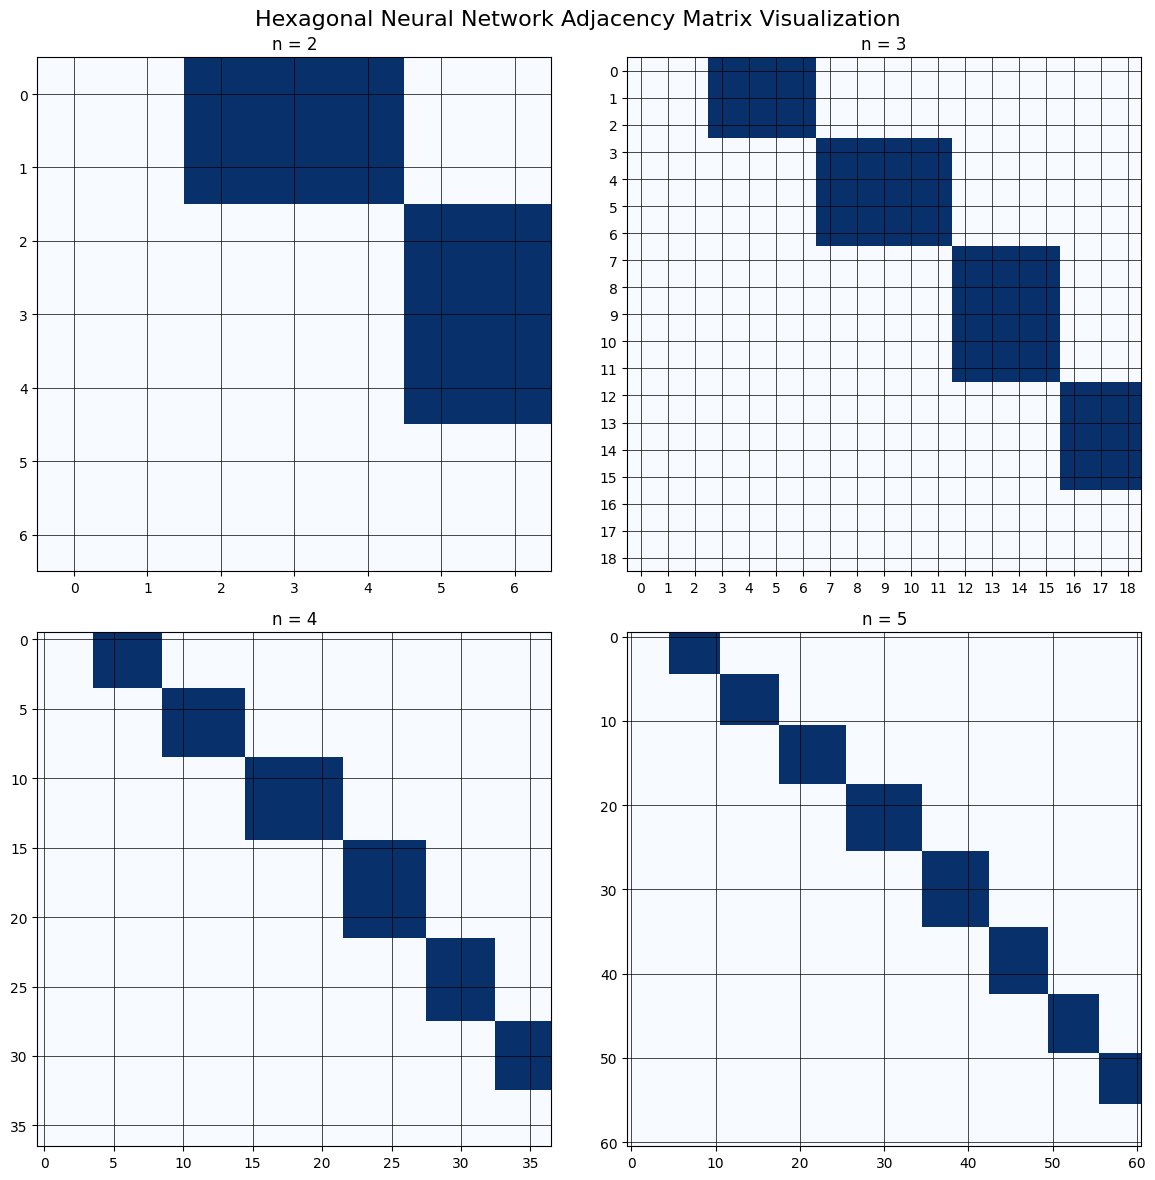
\includegraphics[width=1\linewidth]{adj-matrix-for-h1-on-n234.png}
    \caption{Adjacency Matrix showcasing the Block structure for $H_1$}
    \label{fig:adj-matrix-n234}
\end{figure}

\subsubsection{Example Training Step Flow with $n=2$}

In a network with $n=2$,
\begin{itemize}
    \item The layer sizes are $[2, 3, 2]$
    \item The total number of nodes is $T = 7$
    \item The Weight and Adjacency matrices $A, W \in \mathbb{R}^{7 \times 7}$
    \item The padded input vector $p_0(x)$ is
    \[x_t = \begin{bmatrix}
        x_0 \\
        x_1 \\
        0 \\
        0 \\
        0 \\
        0 \\
        0 \\
    \end{bmatrix}\]

    \item And the padded response vector is
    \[\text{calculated } y_t = \begin{bmatrix}
        0 \\
        0 \\
        0 \\
        0 \\
        0 \\
        y_0 \\
        y_1 \\
    \end{bmatrix}\]
    
\end{itemize}

%%% TODO: add pseudocode for one training step.
%%% TODO: explicitly state optimizer, loss, activation, batching, seed behavior, and update schedule.
%%% TODO: define how gradients on shared weights are accumulated or synchronized.
%%% SUGGESTION: A small Algorithm environment would substantially improve reviewability here.

\subsection{Computational Complexity}

%%% TODO: add asymptotic and practical complexity discussion.
%%% TODO: compare dense global matrix implementation versus block/path implementation.
%%% TODO: include memory complexity for $W \in \mathbb{R}^{T \times T}$ and active orientation blocks.
%%% SUGGESTION: This section is important because the architecture scales badly if represented as dense global matrices.

\subsection{Implementation Reproducibility}

%%% TODO: specify codebase, random seeds, software dependencies, and hardware used for reported runs.
%%% TODO: specify whether results were generated from NumPy reference implementation or another backend.
%%% TODO: specify saved run manifest fields needed to reproduce results.

\subsection{Baseline and Variant Definitions}

%%% SUGGESTION: The following baseline/variant ideas are useful, but they currently read as future experiment notes rather than implemented methods.
%%% SUGGESTION: For a conference paper, either:
%%% SUGGESTION: - move unevaluated variants to Future Work, or
%%% SUGGESTION: - convert this into a clear baseline-definition subsection and only list evaluated baselines.

If we interpret six co-dependent multi layer perceptrons as an ensemble with parameter tying, here are a few variants that we could try finding baselines within the guidance of ensemble based learning \cite{lakshminarayanan2017deep,huang2017snapshot,izmailov2018swa,gal2016dropout}.

We will establish some baseline models, and their expected outputs.
Then we will try five variants of these baselines that are based on exploits and manipulations that we can do exclusively because of hexagonal nature of the graph.
To these five, we will then be testing some orthogonal knobs.  We will establish what are the independent and dependent  and testing variables that we will be fine tuning and sweeping through to test.

First, let's establish some baselines.

\subsubsection{Baselines}

A single model, without sharing, standard training
Deep ensemble, six separate networks, no sharing, independent seeds.
Snapshot ensemble / SWA: 1 network, multi snapshot averaging
MC-Dropout: 1 net, inference-time dropout

%%% TODO: Convert this into a table with columns: baseline, parameter sharing, parameter count, trained orientations, inference rule, purpose.
%%% SUGGESTION: Parameter-count parity should be explicit for every baseline.

\subsubsection{Variants 1 - 5: Hex Ensemble Variants}
Variant 1: Hard Rotation Sharing:
One backbone tensor bank, each member 'applies a hex rotation' to filters adjacency before its forward.
Only small member-specific heads (and optional tiny offsets) are unique.
Combines group equivariance with ensembling

Variant 2: Soft sharing via low-rank delta (LoRA-style)
Shared backbone $\theta$; each member has $\Delta_i = A_iB_i$ (rank-r) on selected layers \cite{hu2022lora}.
Control r to trade diversity vs. parameters
Optimal: permember BN/Layer Norm

Variant 3: Masked weight reuse
Shared tensor bank W; each member uses a binary/ternary mask $M_i$ (learned or fixed) such that $W \circ M_i$
Encourages orthogonal subspaces with negligble memory

Variant 4: Shared backbone, member heads only
Classic multi head: 100 percent sahred feature extractor; six heads (Acts as lower bound on diversity)

Variant 5: Optimizer state-sharing vs isolatioin
Same weights but either (i) one optimizer for all members (cotraining) or (ii) per member optimizers on their delta/heads only.

%%% SUGGESTION: These variants are potentially too many for the first conference paper.
%%% SUGGESTION: A tighter paper may only need:
%%% SUGGESTION: - HexNN single-orientation baseline
%%% SUGGESTION: - parameter-matched MLP
%%% SUGGESTION: - six independent MLPs / ensemble baseline
%%% SUGGESTION: - rotation-scheduled HexNN
%%% SUGGESTION: Leave LoRA/masked/head-only variants to future work unless results already exist.

\section{Data}

%%% SUGGESTION: This section should probably become "Experimental Setup and Benchmark Families" or simply "Experiments" for conference readability.
%%% SUGGESTION: Right now the strongest missing piece is experimental discipline rather than additional ideas.
%%% SUGGESTION: Reviewers will mainly care about:
%%% SUGGESTION: - parameter-count parity
%%% SUGGESTION: - seed count
%%% SUGGESTION: - fair baselines
%%% SUGGESTION: - train/test methodology
%%% SUGGESTION: - whether transfer/interference metrics are rigorously defined

\section{Benchmark Families}

The full cartesian product of all datasets and all known activation patterns, loss functions, learning rate, optimizers now with the new rotation operator would be thorough, it's not quite feasible for the scope of a paper, but it is considered for future work and exhaustive Hexnet dynamic surveying.

Therefore we define a Benchmark Family is a subset of this cartesian product where hold certain hyperparameter constants and test individual themes with thess operators.
The theme of each family along with our findings are detailed below. The datasets are defined afterwards.

%%% SUGGESTION: Existing text: "all known activation patterns"
%%% SUGGESTION: Narrow this wording. Reviewers may interpret it literally.
%%% SUGGESTION: Existing text: "future work and exhaustive Hexnet dynamic surveying"
%%% SUGGESTION: Consider simpler language such as "future exhaustive hyperparameter sweeps".
%%% SUGGESTION: Define benchmark families formally.
%%% TODO: add a benchmark-family table summarizing:
%%% TODO: - family objective
%%% TODO: - datasets
%%% TODO: - fixed variables
%%% TODO: - swept variables
%%% TODO: - evaluation metrics

\subsection{Family A - Linear Structure Recovery}

%%% SUGGESTION: This is probably the correct first benchmark family.
%%% SUGGESTION: Linear and near-linear tasks are good because they isolate topology/scheduling behavior before nonlinear complexity dominates.

Hyper parameters that we will sweep:

\begin{table}
    \centering
    \begin{tabular}{c|c}
        Variable & Options \\
        \hline
        \hline
        Models & hex, mlp \\
        \hline
        Activations & linear, relu, leaky\_relu \\
        \hline
        Losses & mean\_squared\_error, huber \\
        \hline
        Learning Rates & constant, exponential\_decay \\
        \hline
        Dimension & Ladder up by twos, 2, 4, 6, 8 \\
    \end{tabular}
    \label{tab:Benchmark A Hyper parameters}
\end{table}

%%% TODO: add random seed count.
%%% TODO: add optimizer choices.
%%% TODO: add batch size.
%%% TODO: add train/validation/test split policy.
%%% TODO: add rotation schedule variables.
%%% TODO: explicitly state whether MLP baselines are parameter matched.
%%% SUGGESTION: Parameter-count parity may become the single most important reviewer concern.

\begin{table}
    \centering
    \begin{tabular}{c|c}
        Dataset & Notes \\
        \hline
        \hline
        identity & stuff \\
        \hline
        linear\_scale & stuff \\
        \hline
        diagonal\_scale & stuff \\
        \hline
        diagonal\_linear & stuff \\
        \hline
        full\_linear & stuff \\
        \hline
        low\_rank\_linear & stuff \\
        \hline
        affine & stuff \\
        \hline
        orthogonal\_rotation & stuff \\
        \hline
    \end{tabular}
\end{table}

%%% TODO: replace placeholder dataset notes.
%%% TODO: specify exact transformation equations.
%%% TODO: specify dimensionality.
%%% TODO: specify whether data are noisy or noiseless.
%%% TODO: specify sample counts.
%%% TODO: define orthogonal_rotation formally.

This helps us achieve parity with MLP with basic data sets and basic flow validation.
We see hex geometry perform just as well as equivalent MLP architecture, then it may be safe to assume isotropic maps are not trivially penalized.

We also see that on diagonal\_scale, diagonal\_linear, and low\_rank\_linear datasets, Hexnet performs better.

Hex Net loss and regression values fluctuate harshly after the rotation operator is applied, but this interference helps over all loss reach lower optimas on average.

When we specifically tested the orthogonal\_rotation dataset, we noticed that it differed in performance to the other affine transformations encoded in datasets.

%%% SUGGESTION: Move all empirical observations out of Data and into Results.
%%% SUGGESTION: The Data/Experimental Setup section should define methodology, not conclusions.
%%% SUGGESTION: Existing text: "Hexnet performs better"
%%% SUGGESTION: Add statistical framing later:
%%% SUGGESTION: - mean across seeds
%%% SUGGESTION: - variance
%%% SUGGESTION: - effect size
%%% SUGGESTION: - significance if appropriate
%%% SUGGESTION: Existing text: "fluctuate harshly"
%%% SUGGESTION: Replace with measurable language such as oscillatory convergence, transient loss spikes, or synchronization instability.

\subsection{Base Case}
Baselines for $H_0$ have been created where loss function, activation functions, and n are variable, and we can measure their performance with regression metrics such as scalar loss (according to the respective loss function), accuracy (root mean square deviation, as is standard for regression based data sets) and $R^2$ (the coefficient of determination).

%%% SUGGESTION: RMSE is not usually called "accuracy".
%%% SUGGESTION: Use separate regression metrics terminology.
%%% TODO: define all evaluation metrics formally.
%%% TODO: define transfer/interference metrics formally.
%%% TODO: define how cross-orientation evaluation is performed.

\subsection{Rotation Scheduling Families}

%%% TODO: add benchmark-family stubs for:
%%% TODO: - single-orientation training
%%% TODO: - sequential orientation rotation
%%% TODO: - train-one/test-all transfer
%%% TODO: - adjacent vs opposite orientation coupling
%%% TODO: - synchronization interval sweeps
%%% TODO: - EPR sweeps
%%% TODO: - rotation ordering sweeps

%%% SUGGESTION: This may become the most novel empirical contribution of the paper.
%%% SUGGESTION: The scheduling/interference behavior is likely more interesting than raw regression performance.

\subsection{Simulated Data Setup}

I did things here (identity dataset, linear dataset, chat gpt outputted)

%%% TODO: formally define synthetic data generation.
%%% TODO: specify random distributions.
%%% TODO: specify reproducibility seed policy.
%%% TODO: specify whether train/test distributions differ.
%%% SUGGESTION: Avoid mentioning "chat gpt outputted" in the final paper.

\subsection{Real Data Sets}

I did things with real data here

%%% TODO: define every real dataset.
%%% TODO: specify preprocessing.
%%% TODO: specify feature normalization.
%%% TODO: specify why equal-dimensional input/output assumptions remain valid.
%%% TODO: specify train/test split methodology.

\subsection{Baseline Definitions}

%%% TODO: add a baseline comparison table.
%%% TODO: include:
%%% TODO: - parameter count
%%% TODO: - topology
%%% TODO: - shared weights
%%% TODO: - number of subnetworks
%%% TODO: - schedule policy
%%% TODO: - inference procedure

%%% SUGGESTION: You probably do not need many baseline families for the first paper.
%%% SUGGESTION: Strong conference papers often win by having fewer but cleaner experiments.
%%% SUGGESTION: Recommended minimal baseline set:
%%% SUGGESTION: - parameter-matched MLP
%%% SUGGESTION: - HexNN single orientation
%%% SUGGESTION: - HexNN rotation-scheduled
%%% SUGGESTION: - six-independent-network ensemble baseline

\subsection{Experimental Controls}

%%% TODO: explicitly define:
%%% TODO: - parameter-count matching strategy
%%% TODO: - random seed count
%%% TODO: - stopping criteria
%%% TODO: - early stopping policy
%%% TODO: - hardware used
%%% TODO: - runtime budget
%%% TODO: - optimizer settings
%%% TODO: - gradient clipping policy if any
%%% TODO: - learning-rate scheduler policy

%%% SUGGESTION: These controls materially affect review outcomes.
%%% SUGGESTION: Reviewer confidence increases substantially when experiment controls are explicit.

\section{Results}

This is what i got! For continual-learning context, see \cite{kirkpatrick2017overcoming}.


\section{Conclusion}

We introduced hexagonal neural networks as a topology-first variant of layered models and reported early training behavior on baseline tasks.


\section*{Limitations}

%%% SUGGESTION: This paper likely benefits from an explicit limitations section, but keep it short for a conference version.
%%% SUGGESTION: Reviewers will probably question:
%%% SUGGESTION: - scaling cost
%%% SUGGESTION: - whether improvements are due to parameter count differences
%%% SUGGESTION: - whether directional coupling survives larger datasets
%%% SUGGESTION: - whether the architecture materially differs from sparse graph/topology variants

% TODO: discuss computational scaling
% TODO: discuss limited dataset scope
% TODO: discuss uncertainty around generalization beyond synthetic tasks
% TODO: discuss parameter-count parity with MLP baselines

\section*{Future Work}

%%% NOTE: Keep future work tightly coupled to the conference paper's core thesis.
%%% NOTE: Rotational transfer, synchronization schedules, lesioning, and nested-core studies are appropriate.
%%% NOTE: The maze system and Hofstadter/attractor explorations should remain out-of-scope for this paper except perhaps one sentence of broader future directions.

% TODO: rotational scheduling studies
% TODO: transfer/interference matrices
% TODO: nested-core initialization
% TODO: lesioning studies
% TODO: PyTorch and large-scale benchmarking backend
% TODO: synchronization strategies and multi-rotation training

\printbibliography

\end{document}